%OBAL
\thispagestyle{empty}
\begin{center}
  \textsc{ 
    {\Large \school\\ \faculty}
    \vfill
    {\LARGE \title}\\ \vspace{0.5cm}
    {\large \thesis}
  }
\end{center}
\vfill

\begin{flushleft}
  \year\\
  \hspace{0.5cm} \author
\end{flushleft}


%TITULNY LIST
\thispagestyle{empty}
\begin{center}
  \textsc{ 
    {\Large \school\\ \faculty}
    \vfill
    {\LARGE \title}\\ \vspace{0.5cm}
    {\large \thesis}
  }
\end{center}
\vfill

\begin{flushleft}
  \begin{tabular}{@{}ll}
    Study programme: & \studyprogramme \\
    Study field: & \studyfield \\
	  Department: & \department \\
    Supervisor: & \supervisor
  \end{tabular}
  \vspace{1cm}

  \placeandyear\\
  \hspace{0.5cm} \author
\end{flushleft}



\shorthandoff{-} %docasne deaktivuje znak '-' v balicku babel
%ZADANIE EN
% 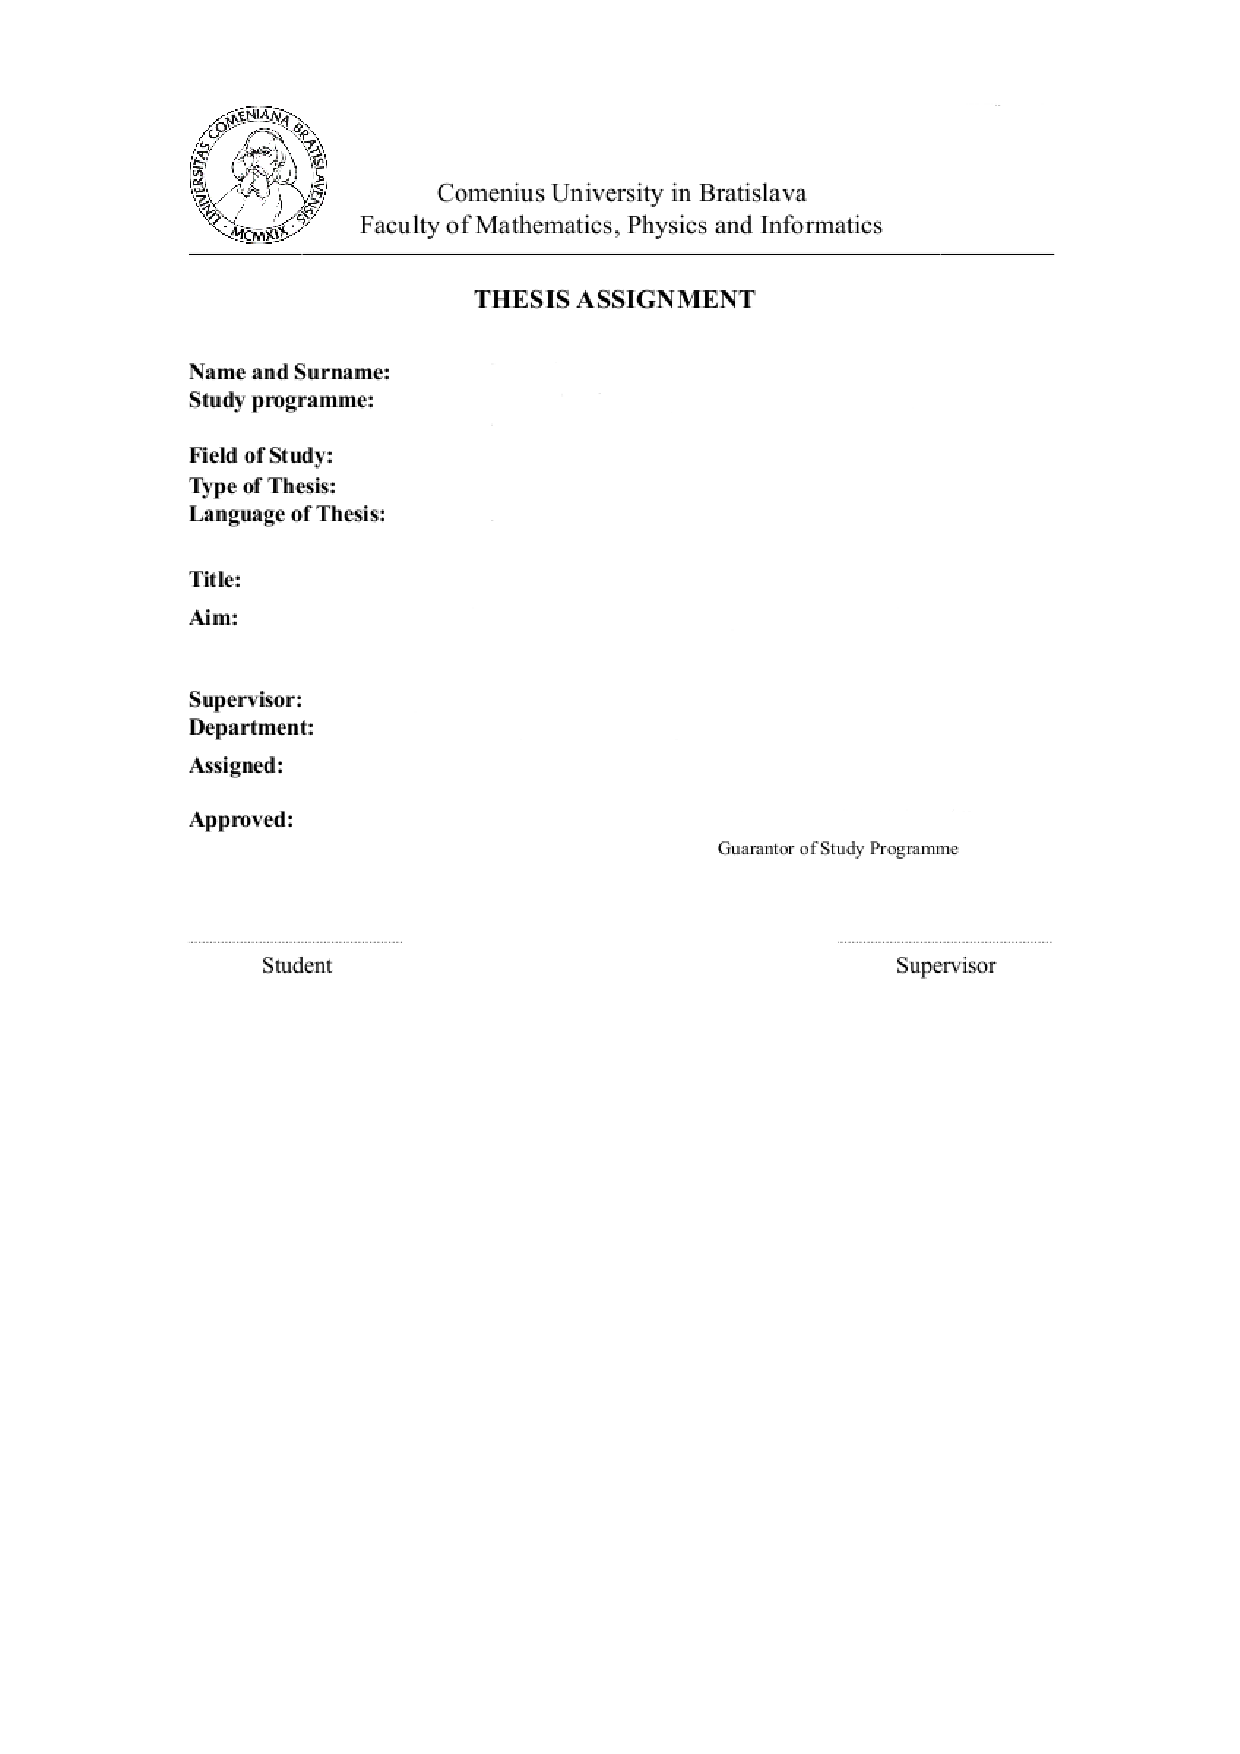
\includepdf[pages=-]{frontmatter/assignment.pdf}
%ZADANIE SK
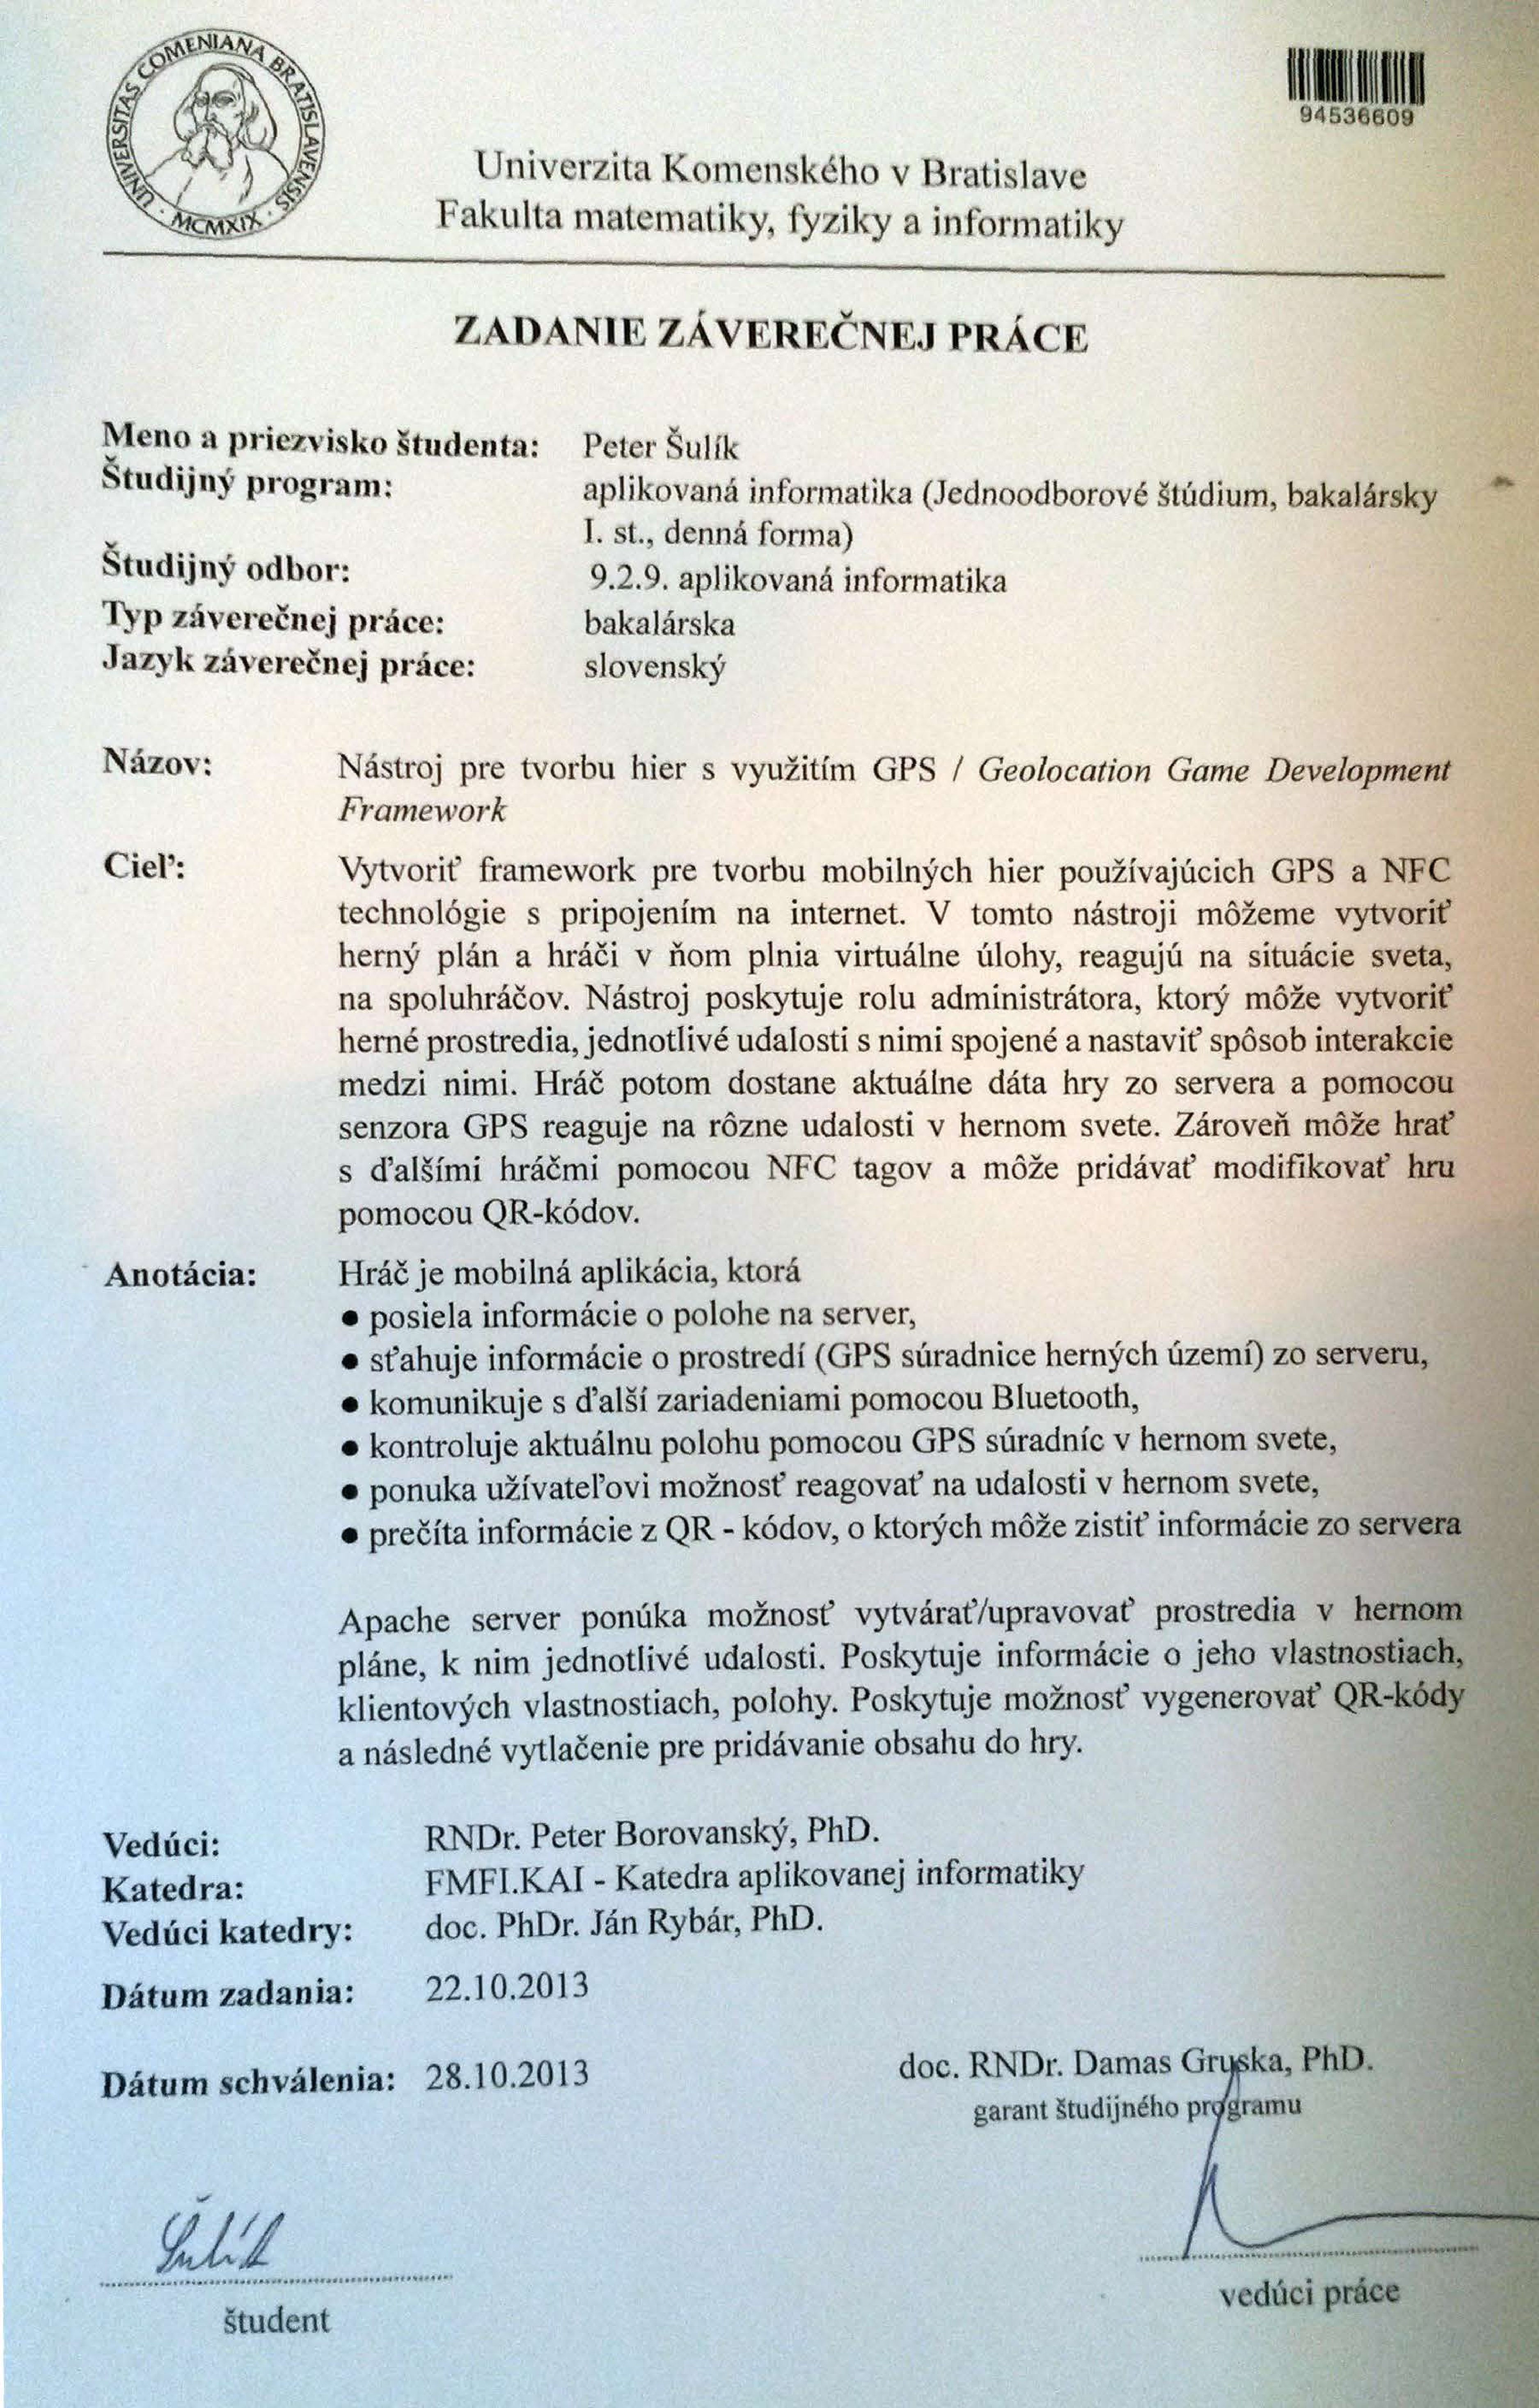
\includepdf[pages=-]{frontmatter/zadanie.pdf}
\shorthandon{-}

\selectlanguage{slovak}
Čestne prehlasujem, že som túto bakalársku prácu vypracoval samostatne s použitím uvedených zdrojov a literatúry.

\null
\vfill
V Bratislave dňa \
30.5. 2014


%PODAKOVANIE
\chapter{Poďakovanie}
\vfil
Chcel by som sa poďakovať svojmu školiteľovi RNDr. Petrovi Borovanskému, PhD. za cenné rady a pripomienky pri tvorbe tejto bakalárskej práce a svojej rodine a priateľom za podporu.


%ABSTRAKT SK
\selectlanguage{slovak}
\chapter{Abstrakt}
Vytvoriť framework pre tvorbu mobilných hier používajúcich GPS a NFC technológie s pripojením na internet. V tomto nástroji môžeme vytvoriť herný plán a hráči v ňom plnia virtuálne úlohy, reagujú na situácie sveta, na spoluhráčov. Nástroj poskytuje rolu administrátora, ktorý môže vytvoriť herné prostredia, jednotlivé udalosti s nimi spojené a nastaviť spôsob interakcie medzi nimi. Hráč potom dostane aktuálne dáta hry zo servera a pomocou senzora GPS reaguje na rôzne udalosti v hernom svete. Zároveň môže hrať s ďalšími hráčmi pomocou NFC tagov a môže pridávať modifikovať hru pomocou QR-kódov.\\ \\
\textbf{\textsc{Kľúčové slová:}} GPS, Android, Multiplayer, Hra, Framework


%ABSTRAKT EN
\selectlanguage{english}
{\noindent\large\bf Abstrakt}

\vspace{1.8cm}

Tu je text slovenskej verzie abstraktu
\\

{\parindent0pt \textbf{Kľúčové slová:} \emph{slovo1, slovo2, slovo3, slovo4}} 

\newpage
 {\noindent\large\bf Abstract}
  \vspace{1.8cm}
 

Text anglickej verzie abstraktu
\\

{\parindent0pt \textbf{Keywords:} \emph{word1, word2, word3, word4}}


\newpage


\selectlanguage{slovak}

%PREDHOVOR
% \chapter{Predhovor beetaa}

\paragraph{Na začiatku bola myšlienka}
Lepší svet.\
Vývoj moderných technológii napreduje čoraz rýchlejším tempom a otvára nám množstvo možností. Mnohé technológie, ktoré dnes považujeme za samozrejmosť a tažko by sa mnohým bez nich predstavoval život, pred pár dekádami boli iba ďalekým zhlukom myšlienok či divokých pribehov science-fiction. Dnes žijeme v týchto príbehoch. \

Behom pár kliknútí môžeme komunikovať s ľudmi na druhej strane Zeme. Možeme jednoduchým stiskom tlačítka zväčniť momenty a zážitky. Dokážeme lepšie liečiť. Tvoriť

Bohužial výdobitky pokroku, ktoré vznikli preto aby spravili svet lepším sú mnohokrát zneužité a ďaleko od svojho pôvodného učelu. Mnohokrát to čo malo pomáhať a tvoriť iba ubližuje a níčí. A stlačením tlačítka sa dá zničiť množstvo životov. \


S technologickým pokrokom sa nám ponúka viac možností a väčšia moc. Svet nebude lepší vďaka rýchlejším kvantovým počítačom, nanotechnológiam, medzihviezdnemu cestovaniu ani žiadnemu inému techologickému pokroku. Svet však môže byť lepší. Ak to dokážeme my ľudia k sebe.



 % Ak ukážeme, že vieme čo znamená byť humánnym a lepším.







%OBSAH
\tableofcontents

%ZOZNAM ILUSTRACII
\listoffigures

%ZOZNAM TABULIEK
%\listoftables
